\documentclass[aspectratio=169,10pt]{beamer}
\usetheme{Madrid}
\usecolortheme{seahorse}
\usepackage{fontspec}
\setsansfont{Noto Sans}
\setmonofont{Noto Sans Mono}[Scale=0.87]
\usepackage{booktabs,tabularx,array,multicol,amsmath}
\usepackage{tikz}
\usetikzlibrary{positioning,arrows.meta,shapes.geometric,calc}
\usepackage{listings}
\usepackage{xcolor}
\usepackage{hyperref}
\definecolor{NEUBlue}{HTML}{16436B}
\definecolor{NEUGreen}{HTML}{087056}
\definecolor{NEUPale}{HTML}{EFF5FA}
\definecolor{SQLBlue}{HTML}{114EAA}
\definecolor{SQLGreen}{HTML}{08704D}
\definecolor{SQLGray}{HTML}{5B6574}
\definecolor{SQLBG}{HTML}{F7FAFD}
\definecolor{NEURed}{HTML}{A82F38}
\setbeamercolor{structure}{fg=NEUBlue}
\setbeamercolor{frametitle}{fg=white,bg=NEUBlue}
\setbeamercolor{title}{fg=white,bg=NEUBlue}
\setbeamercolor{block title}{bg=NEUBlue,fg=white}
\setbeamercolor{block body}{bg=NEUPale,fg=black}
\setbeamercolor{alertblock title}{bg=NEURed,fg=white}
\setbeamercolor{alertblock body}{bg=red!5,fg=black}
\setbeamertemplate{navigation symbols}{}
\setbeamertemplate{footline}[frame number]
\setbeamertemplate{itemize items}[circle]
\setbeamertemplate{blocks}[rounded][shadow=false]
\setbeamersize{text margin left=.85cm,text margin right=.85cm}
\lstdefinelanguage{MySQL}{
morekeywords={SELECT,FROM,WHERE,AS,DISTINCT,ORDER,BY,ASC,DESC,LIMIT,OFFSET,AND,OR,NOT,LIKE,IN,BETWEEN,IS,NULL,JOIN,INNER,LEFT,RIGHT,CROSS,ON,COUNT,SUM,AVG,MIN,MAX,GROUP,HAVING,CASE,WHEN,THEN,ELSE,END,IF,IFNULL,COALESCE,NULLIF,CONCAT,USE,SHOW,TABLES,DESC,DESCRIBE,WITH,RECURSIVE,UNION,ALL,EXPLAIN,TRUE,FALSE},
sensitive=false,morecomment=[l]{--},morestring=[b]' }
\lstdefinestyle{sql}{language=MySQL,basicstyle=\ttfamily\footnotesize,keywordstyle=\color{SQLBlue}\bfseries,commentstyle=\color{SQLGray},stringstyle=\color{SQLGreen},backgroundcolor=\color{SQLBG},frame=single,rulecolor=\color{black!18},columns=fullflexible,keepspaces=true,breaklines=true,breakatwhitespace=true,showstringspaces=false,xleftmargin=.35em,xrightmargin=.35em,aboveskip=.4em,belowskip=.3em}
\lstset{style=sql}
\newcommand{\code}[1]{\texttt{#1}}
\newcommand{\kw}[1]{\textcolor{NEUBlue}{\bfseries #1}}
\title[SQL SELECT 6]{CTE và WITH RECURSIVE trong MySQL}
\subtitle{DBMS -- SELECT Statement 6}
\author{DBMS Course}
\institute{Smart Logistics and Supply Chain Management Lab}
\date{2026}
\begin{document}
\begin{frame}[fragile]{SELECT 6: Common Table Expressions (CTE)}

\vspace{.65cm}
\begin{center}
{\Huge\bfseries CTE và \texttt{WITH RECURSIVE}}\\[.35cm]
{\large Cú pháp -- Phân tích -- Ví dụ \texttt{classicmodels} -- Bài tập}\\[.65cm]
{\small DBMS Course \quad|\quad MySQL 8+ \quad|\quad 2026}
\end{center}
\end{frame}

\begin{frame}[fragile]{Mục tiêu học tập}
\small
\begin{itemize}
\item Giải thích CTE là gì, phạm vi sử dụng và lợi ích khi chia truy vấn.
\item Viết \code{WITH} kết hợp \code{WHERE}, \code{ORDER BY}, \code{LIMIT}.
\item Tạo CTE có \code{GROUP BY} và nối kết quả với các bảng khác.
\item Khai báo nhiều CTE để xây dựng báo cáo theo từng bước.
\item Viết \code{WITH RECURSIVE} duyệt cây quản lý nhân viên.
\item Phân tích lỗi và hạn chế của CTE, nhất là CTE đệ quy.
\end{itemize}
\end{frame}

\begin{frame}[fragile]{Lộ trình bài học}

\begin{center}
\begin{tikzpicture}[node distance=.50cm and .45cm,>=Latex,
 n/.style={draw=NEUBlue,thick,rounded corners,fill=NEUPale,minimum width=3.20cm,minimum height=1.12cm,align=center,font=\small}]
\node[n] (a) {CTE là gì?\\Cú pháp \texttt{WITH}};
\node[n,right=of a] (b) {Lọc, sắp xếp\\\texttt{WHERE / LIMIT}};
\node[n,right=of b] (c) {Tổng hợp\\\texttt{GROUP BY}};
\node[n,below=1cm of c] (d) {CTE với \texttt{JOIN}};
\node[n,left=of d] (e) {Nhiều CTE\\trong một \texttt{WITH}};
\node[n,left=of e] (f) {\texttt{WITH RECURSIVE}\\Cây nhân viên};
\draw[->,thick,NEUGreen](a)--(b);\draw[->,thick,NEUGreen](b)--(c);
\draw[->,thick,NEUGreen](c)--(d);\draw[->,thick,NEUGreen](d)--(e);
\draw[->,thick,NEUGreen](e)--(f);
\end{tikzpicture}
\end{center}
\end{frame}

\section{CSDL mẫu và nền tảng}

\begin{frame}[fragile]{Các bảng trong classicmodels}
\small
\begin{center}
\begin{tabular}{l p{7.2cm}}
\toprule
Bảng & Vai trò \\
\midrule
\code{customers} & Khách hàng \\
\code{orders} & Đơn hàng \\
\code{orderdetails} & Chi tiết từng sản phẩm đặt hàng \\
\code{payments} & Thanh toán \\
\code{products} & Sản phẩm \\
\code{productlines} & Dòng sản phẩm \\
\code{employees} & Nhân viên và quản lý \\
\code{offices} & Văn phòng \\
\bottomrule
\end{tabular}
\end{center}
\vspace{.25em}
\small Bộ slide sử dụng \textbf{tên cột của schema classicmodels}; số liệu trong những bảng ví dụ nhỏ được ghi rõ là minh họa.
\end{frame}

\begin{frame}[fragile]{Các khóa dùng nhiều trong bài}
\small
\begin{center}
\begin{tabular}{l l l}
\toprule
Bảng nguồn & Cột liên kết & Bảng đích \\
\midrule
\code{orders} & \code{customerNumber} & \code{customers} \\
\code{payments} & \code{customerNumber} & \code{customers} \\
\code{orderdetails} & \code{orderNumber} & \code{orders} \\
\code{orderdetails} & \code{productCode} & \code{products} \\
\code{customers} & \code{salesRepEmployeeNumber} & \code{employees} \\
\code{employees} & \code{reportsTo} & \code{employees} \\
\bottomrule
\end{tabular}
\end{center}
\vspace{.25em}
\begin{block}{Với cây quản lý}\code{employees.reportsTo} trỏ đến \code{employees.employeeNumber}: đây là quan hệ \textbf{tự tham chiếu}.\end{block}
\end{frame}

\begin{frame}[fragile]{Khởi động MySQL: kiểm tra schema}
\small
\begin{lstlisting}[basicstyle=\ttfamily\footnotesize]
USE classicmodels;
SHOW TABLES;
DESC customers;
DESC payments;
DESC orders;
DESC orderdetails;
DESC employees;
\end{lstlisting}
\vspace{.1em}
\begin{itemize}
\item \code{USE}: chọn CSDL.
\item \code{DESC}: đọc tên cột, kiểu dữ liệu, khóa và khả năng \code{NULL}.
\item Không cần tự đoán tên cột khi viết \code{SELECT} hoặc \code{JOIN}.
\end{itemize}
\end{frame}

\section{CTE thường với WITH}

\begin{frame}[fragile]{CTE là gì?}
\small
\begin{itemize}
\item CTE = \emph{Common Table Expression}: biểu thức bảng được đặt tên.
\item Được khai báo bằng \code{WITH} ngay trước câu lệnh dùng nó.
\item Có thể tham chiếu tên CTE trong truy vấn chính như tham chiếu bảng.
\item CTE thông thường chỉ tồn tại trong \textbf{phạm vi một câu lệnh}, không tạo bảng vĩnh viễn.
\end{itemize}
\vspace{.3em}\begin{block}{Điểm cần nhớ}
CTE giúp phân tách bài toán thành các bước có tên rõ nghĩa; \textbf{không mặc nhiên nhanh hơn} subquery hoặc JOIN.
\end{block}
\end{frame}

\begin{frame}[fragile]{Cú pháp CTE thường}
\small
\begin{lstlisting}[basicstyle=\ttfamily\footnotesize]
WITH cte_name AS (
    SELECT col1, col2, ...
    FROM source_table
    WHERE condition
)
SELECT col1, col2
FROM cte_name;
\end{lstlisting}
\vspace{.1em}
\begin{itemize}
\item \code{WITH}: bắt đầu khai báo CTE.
\item \code{cte\_name}: tên kết quả trung gian.
\item \code{AS (SELECT ...)}: định nghĩa kết quả mà CTE biểu diễn.
\item \code{SELECT ... FROM cte\_name}: câu truy vấn chính sử dụng CTE.
\end{itemize}
\end{frame}

\begin{frame}[fragile]{CTE được sử dụng như thế nào?}

\begin{center}
\begin{tikzpicture}[>=Latex,node distance=1.15cm,box/.style={draw=NEUBlue,rounded corners,thick,fill=NEUPale,text width=3.05cm,minimum height=1.26cm,align=center}]
\node[box] (a) {Bảng \texttt{customers}\\(dữ liệu gốc)};
\node[box,right=of a] (b) {CTE \texttt{usa\_customers}\\\texttt{WHERE country='USA'}};
\node[box,right=of b] (c) {Truy vấn chính\\\texttt{creditLimit}\\\texttt{>100000}};
\draw[->,thick,NEUGreen] (a)--(b);
\draw[->,thick,NEUGreen] (b)--(c);
\end{tikzpicture}
\end{center}
\begin{alertblock}{Chú ý}
Sơ đồ mô tả \textbf{logic truy vấn}; optimizer của MySQL có thể gộp hoặc thực thi CTE theo kế hoạch khác.
\end{alertblock}
\end{frame}

\begin{frame}[fragile]{Ví dụ 1: khách hàng ở USA}
\small
\begin{lstlisting}[basicstyle=\ttfamily\scriptsize]
WITH usa_customers AS (
    SELECT customerNumber, customerName,
           city, country, creditLimit
    FROM customers
    WHERE country = 'USA'
)
SELECT customerNumber, customerName,
       creditLimit
FROM usa_customers;
\end{lstlisting}
\vspace{.1em}
\begin{itemize}
\item CTE \code{usa\_customers} chứa những dòng của \code{customers} ở USA.
\item Các cột trong SELECT cuối lấy từ \code{usa\_customers}.
\item Có thể thay danh sách cột bằng \code{SELECT *} khi khám phá dữ liệu.
\end{itemize}
\end{frame}

\begin{frame}[fragile]{Ví dụ 2: lọc thêm sau CTE}
\small
\begin{lstlisting}[basicstyle=\ttfamily\scriptsize]
WITH usa_customers AS (
    SELECT customerNumber, customerName,
           country, creditLimit
    FROM customers
    WHERE country = 'USA'
)
SELECT customerName, creditLimit
FROM usa_customers
WHERE creditLimit > 100000;
\end{lstlisting}
\vspace{.1em}
\begin{itemize}
\item Điều kiện trong CTE: \code{country = 'USA'}.
\item Điều kiện ngoài CTE: \code{creditLimit} $>100000$.
\item Có thể đọc truy vấn thành hai bước logic: \emph{chọn khách USA, rồi lọc hạn mức}.
\end{itemize}
\end{frame}

\begin{frame}[fragile]{Ví dụ 3: sản phẩm Classic Cars}
\small
\begin{lstlisting}[basicstyle=\ttfamily\scriptsize]
WITH classic_cars AS (
    SELECT productCode, productName,
           productLine, MSRP
    FROM products
    WHERE productLine = 'Classic Cars'
)
SELECT productCode, productName, MSRP
FROM classic_cars
ORDER BY MSRP DESC;
\end{lstlisting}
\vspace{.1em}
\begin{itemize}
\item Bảng nguồn: \code{products}.
\item Cột điều kiện: \code{products.productLine}.
\item Cột kết quả: \code{productCode}, \code{productName}, \code{MSRP}.
\end{itemize}
\end{frame}

\begin{frame}[fragile]{Ví dụ 4: CTE đơn hàng đã giao}
\small
\begin{lstlisting}[basicstyle=\ttfamily\scriptsize]
WITH shipped_orders AS (
    SELECT orderNumber, orderDate,
           shippedDate, status, customerNumber
    FROM orders
    WHERE status = 'Shipped'
)
SELECT orderNumber, orderDate, customerNumber
FROM shipped_orders
WHERE orderDate >= '2005-01-01';
\end{lstlisting}
\vspace{.1em}
\begin{itemize}
\item CTE được tạo từ \code{orders}.
\item Điều kiện ngày dùng so sánh với giá trị kiểu ngày (\code{DATE}).
\item Trong dữ liệu thực tế cần hiểu rõ ý nghĩa của \code{orderDate} và \code{shippedDate}.
\end{itemize}
\end{frame}

\begin{frame}[fragile]{CTE thường, bảng dẫn xuất và VIEW}
\begin{columns}[T,onlytextwidth]
\column{.49\textwidth}
\begin{block}{CTE}
\small
\begin{itemize}
\item Có tên ngay trong câu lệnh.
\item Dùng lại nhiều lần trong câu lệnh đó.
\item Không tồn tại sau khi câu lệnh kết thúc.
\end{itemize}
\end{block}
\column{.49\textwidth}
\begin{block}{Derived table / VIEW}
\small
\begin{itemize}
\item Derived table: subquery trong \texttt{FROM}, cần bí danh.
\item VIEW: đối tượng lược đồ được lưu bằng \texttt{CREATE VIEW}.
\item Không đồng nhất với việc tạo bảng vật lý.
\end{itemize}
\end{block}
\end{columns}
\vspace{.3em}
\small Chọn hình thức nào tùy mục tiêu: dễ đọc, khả năng tái sử dụng, và cách optimizer xử lý.
\end{frame}

\section{CTE + lọc và sắp xếp}

\begin{frame}[fragile]{CTE với ORDER BY và LIMIT}
\small
\begin{lstlisting}[basicstyle=\ttfamily\scriptsize]
WITH motorcycles AS (
    SELECT productCode, productName, MSRP
    FROM products
    WHERE productLine = 'Motorcycles'
)
SELECT productCode, productName, MSRP
FROM motorcycles
ORDER BY MSRP DESC
LIMIT 5;
\end{lstlisting}
\vspace{.1em}
\begin{itemize}
\item \code{ORDER BY MSRP DESC}: giá đề xuất giảm dần.
\item \code{LIMIT 5}: chỉ trả về 5 dòng đầu theo thứ tự đó.
\item Thêm tiêu chí phụ, chẳng hạn \code{productCode}, nếu muốn phá hòa một cách nhất quán.
\end{itemize}
\end{frame}

\begin{frame}[fragile]{CTE lọc theo năm 2004: payments}
\small
\begin{lstlisting}[basicstyle=\ttfamily\scriptsize]
WITH payments_2004 AS (
    SELECT customerNumber, checkNumber,
           paymentDate, amount
    FROM payments
    WHERE paymentDate >= '2004-01-01'
      AND paymentDate <  '2005-01-01'
)
SELECT checkNumber, paymentDate, amount
FROM payments_2004
ORDER BY amount DESC
LIMIT 5;
\end{lstlisting}
\vspace{.1em}
\begin{itemize}
\item Cách lọc \textbf{nửa khoảng} thường dễ hiểu và áp dụng tốt cho cột ngày/giờ.
\item \code{amount} là cột gốc của \code{payments}; không phải giá trị tổng hợp.
\end{itemize}
\end{frame}

\begin{frame}[fragile]{CTE tồn kho thấp}
\small
\begin{lstlisting}[basicstyle=\ttfamily\scriptsize]
WITH low_stock AS (
    SELECT productCode, productName,
           quantityInStock
    FROM products
    WHERE quantityInStock < 1000
)
SELECT productCode, productName,
       quantityInStock
FROM low_stock
ORDER BY quantityInStock ASC;
\end{lstlisting}
\vspace{.1em}
\begin{itemize}
\item Tên CTE mô tả ý nghĩa điều kiện trong truy vấn con.
\item Kết quả có thể trống nếu CSDL hiện tại không có sản phẩm nào dưới ngưỡng.
\end{itemize}
\end{frame}

\begin{frame}[fragile]{Thực hành 1: top 5 sản phẩm}
\begin{block}{Yêu cầu}
Dùng một CTE để lấy \textbf{5 sản phẩm Motorcycles có MSRP cao nhất}. Cột cần trả: \code{productCode}, \code{productName}, \code{MSRP}.
\end{block}
\begin{alertblock}{Gợi ý làm bài}
CTE đọc từ \code{products}; truy vấn chính dùng \code{ORDER BY MSRP DESC LIMIT 5}.
\end{alertblock}
\textbf{Đáp án tham khảo (rút gọn):}
\begin{lstlisting}[basicstyle=\ttfamily\scriptsize]
WITH mc AS (
  SELECT productCode, productName, MSRP
  FROM products WHERE productLine='Motorcycles'
)
SELECT * FROM mc ORDER BY MSRP DESC LIMIT 5;
\end{lstlisting}
\end{frame}

\section{CTE + hàm tổng hợp}

\begin{frame}[fragile]{Vì sao dùng CTE để tổng hợp?}
\small
\begin{itemize}
\item Tách phần \emph{tính toán theo nhóm} khỏi phần trình bày hoặc lọc kết quả.
\item Giúp đưa \code{SUM}, \code{COUNT}, \code{AVG} vào một kết quả trung gian có tên.
\item Dễ nối tổng hợp với \code{customers}, \code{orders}, \code{products}.
\item Tên cột suy ra từ hàm tổng hợp cần đặt bằng \code{AS}, ví dụ \code{totalPayment}.
\end{itemize}
\vspace{.3em}\begin{block}{Điểm cần nhớ}
Một dòng của CTE tổng hợp có thể đại diện cho \textbf{một khách hàng / một đơn hàng / một sản phẩm}, không còn là một dòng giao dịch.
\end{block}
\end{frame}

\begin{frame}[fragile]{Cú pháp: tổng hợp bên trong CTE}
\small
\begin{lstlisting}[basicstyle=\ttfamily\scriptsize]
WITH summary AS (
    SELECT group_key,
           SUM(amount_column) AS total_amount
    FROM source_table
    GROUP BY group_key
)
SELECT group_key, total_amount
FROM summary
WHERE total_amount > threshold;
\end{lstlisting}
\vspace{.1em}
\begin{itemize}
\item \code{group\_key}: khóa định danh mỗi nhóm.
\item \code{SUM}: tạo giá trị tổng hợp cho nhóm.
\item Bên ngoài CTE có thể lọc trực tiếp cột đã đặt bí danh.
\end{itemize}
\end{frame}

\begin{frame}[fragile]{Tổng thanh toán theo khách hàng}
\small
\begin{lstlisting}[basicstyle=\ttfamily\scriptsize]
WITH payment_summary AS (
    SELECT customerNumber,
           SUM(amount) AS totalPayment
    FROM payments
    GROUP BY customerNumber
)
SELECT customerNumber, totalPayment
FROM payment_summary
ORDER BY totalPayment DESC;
\end{lstlisting}
\vspace{.1em}
\begin{itemize}
\item \code{payments.amount}: số tiền của từng khoản thanh toán.
\item \code{GROUP BY customerNumber}: một dòng / khách hàng có thanh toán.
\item \code{totalPayment}: cột \textbf{tính toán}, không có sẵn trong \code{payments}.
\end{itemize}
\end{frame}

\begin{frame}[fragile]{Từ giao dịch sang kết quả tổng hợp}

\small
\begin{columns}[T,onlytextwidth]
\column{.47\textwidth}
\textbf{payments (minh họa)}
\begin{tabular}{l r}
\toprule
customerNumber & amount\\\midrule
101 & 200\\
101 & 350\\
102 & 180\\
102 & 120\\
\bottomrule
\end{tabular}
\column{.47\textwidth}
\textbf{payment\_summary (minh họa)}
\begin{tabular}{l r}
\toprule
customerNumber & totalPayment\\\midrule
101 & 550\\
102 & 300\\
\bottomrule
\end{tabular}
\end{columns}
\vspace{.35cm}
\begin{block}{Chuyển đổi số dòng}
\texttt{GROUP BY customerNumber} gom nhiều bản ghi thanh toán thành một nhóm; \texttt{SUM(amount)} tính tổng của từng nhóm.
\end{block}
\end{frame}

\begin{frame}[fragile]{Doanh thu từng đơn hàng}
\small
\begin{lstlisting}[basicstyle=\ttfamily\scriptsize]
WITH order_summary AS (
    SELECT orderNumber,
           SUM(quantityOrdered * priceEach)
             AS orderTotal
    FROM orderdetails
    GROUP BY orderNumber
)
SELECT orderNumber, orderTotal
FROM order_summary
WHERE orderTotal > 50000
ORDER BY orderTotal DESC;
\end{lstlisting}
\vspace{.1em}
\begin{itemize}
\item \code{quantityOrdered}, \code{priceEach} thuộc bảng \code{orderdetails}.
\item \code{orderTotal}: tổng \code{quantityOrdered * priceEach} của các dòng cùng \code{orderNumber}.
\item Điều kiện ngưỡng áp dụng sau khi đã có CTE tổng hợp.
\end{itemize}
\end{frame}

\begin{frame}[fragile]{Số đơn hàng theo khách hàng}
\small
\begin{lstlisting}[basicstyle=\ttfamily\scriptsize]
WITH order_count AS (
    SELECT customerNumber,
           COUNT(*) AS numberOfOrders
    FROM orders
    GROUP BY customerNumber
)
SELECT customerNumber, numberOfOrders
FROM order_count
WHERE numberOfOrders > 5;
\end{lstlisting}
\vspace{.1em}
\begin{itemize}
\item Bảng \code{orders}: mỗi hàng tương ứng một đơn hàng.
\item \code{COUNT(*)}: đếm số đơn hàng của mỗi khách hàng.
\item Không có hàng tổng hợp cho khách chưa từng đặt hàng (nếu không nối với bảng khách hàng).
\end{itemize}
\end{frame}

\begin{frame}[fragile]{Thực hành 2: tổng tiền theo đơn hàng}
\begin{block}{Yêu cầu}
Cho \code{orderdetails(orderNumber, productCode, quantityOrdered, priceEach)}. Tính \code{orderTotal} cho từng \code{orderNumber} bằng CTE.
\end{block}
\begin{alertblock}{Gợi ý làm bài}
Gom nhóm theo \code{orderNumber}; tính \code{SUM(quantityOrdered * priceEach)}.
\end{alertblock}
\textbf{Đáp án tham khảo (rút gọn):}
\begin{lstlisting}[basicstyle=\ttfamily\scriptsize]
WITH order_summary AS (
  SELECT orderNumber,
    SUM(quantityOrdered*priceEach) AS orderTotal
  FROM orderdetails GROUP BY orderNumber
)
SELECT * FROM order_summary;
\end{lstlisting}
\end{frame}

\section{CTE và JOIN}

\begin{frame}[fragile]{Khi nào JOIN với CTE?}
\small
\begin{itemize}
\item CTE giữ \textbf{chỉ số tổng hợp}; bảng gốc giữ \textbf{thông tin mô tả}.
\item Khóa của CTE tổng hợp phải đủ để nối, ví dụ \code{customerNumber}.
\item Dùng \code{INNER JOIN} khi chỉ muốn các thực thể có dữ liệu tổng hợp.
\item Dùng \code{LEFT JOIN} nếu muốn giữ thực thể chưa phát sinh giao dịch.
\end{itemize}
\vspace{.3em}\begin{block}{Điểm cần nhớ}
Tránh nối dữ liệu chi tiết với dữ liệu tổng hợp theo khóa không duy nhất, vì dễ nhân số dòng và làm sai tổng.
\end{block}
\end{frame}

\begin{frame}[fragile]{CTE tổng thanh toán + customers}
\small
\begin{lstlisting}[basicstyle=\ttfamily\scriptsize]
WITH payment_summary AS (
    SELECT customerNumber,
           SUM(amount) AS totalPayment
    FROM payments
    GROUP BY customerNumber
)
SELECT c.customerNumber,
       c.customerName, ps.totalPayment
FROM customers AS c
JOIN payment_summary AS ps
  ON c.customerNumber = ps.customerNumber;
\end{lstlisting}
\vspace{.1em}
\begin{itemize}
\item \code{customerName}: cột nguồn \code{customers}.
\item \code{totalPayment}: cột tổng hợp của CTE \code{payment\_summary}.
\item \code{ON}: hai phía nối cùng khóa \code{customerNumber}.
\end{itemize}
\end{frame}

\begin{frame}[fragile]{CTE doanh thu + đơn hàng + khách hàng}
\small
\begin{lstlisting}[basicstyle=\ttfamily\scriptsize]
WITH order_summary AS (
    SELECT orderNumber,
           SUM(quantityOrdered * priceEach) AS orderTotal
    FROM orderdetails
    GROUP BY orderNumber
)
SELECT o.orderNumber, o.orderDate,
       c.customerName, os.orderTotal
FROM orders AS o
JOIN customers AS c
  ON o.customerNumber = c.customerNumber
JOIN order_summary AS os
  ON o.orderNumber = os.orderNumber;
\end{lstlisting}
\vspace{.1em}
\begin{itemize}
\item \code{orders}: mã đơn, ngày đặt, mã khách.
\item \code{customers}: tên khách.
\item \code{order\_summary}: tổng tiền theo từng đơn.
\end{itemize}
\end{frame}

\begin{frame}[fragile]{INNER JOIN hay LEFT JOIN với CTE?}
\begin{columns}[T,onlytextwidth]
\column{.49\textwidth}
\begin{block}{INNER JOIN}
\small
\begin{itemize}
\item Chỉ giữ khách hàng có bản ghi tổng hợp phù hợp.
\item Khách không có thanh toán không xuất hiện.
\end{itemize}
\end{block}
\column{.49\textwidth}
\begin{block}{LEFT JOIN}
\small
\begin{itemize}
\item Giữ tất cả khách hàng từ \texttt{customers}.
\item \texttt{totalPayment} là \texttt{NULL} nếu không có thanh toán.
\item Có thể dùng \texttt{COALESCE(...,0)} khi cần hiển thị 0.
\end{itemize}
\end{block}
\end{columns}
\end{frame}

\begin{frame}[fragile]{LEFT JOIN + COALESCE: cả khách chưa thanh toán}
\small
\begin{lstlisting}[basicstyle=\ttfamily\scriptsize]
WITH pay AS (
    SELECT customerNumber,
           SUM(amount) AS totalPayment
    FROM payments GROUP BY customerNumber
)
SELECT c.customerNumber, c.customerName,
       COALESCE(pay.totalPayment, 0)
         AS totalPayment
FROM customers AS c
LEFT JOIN pay
  ON c.customerNumber = pay.customerNumber;
\end{lstlisting}
\vspace{.1em}
\begin{itemize}
\item \code{COALESCE(..., 0)} biến \code{NULL} (không có giá trị tổng hợp) thành 0 để hiển thị.
\item \textbf{Phân biệt:} không có thanh toán và thanh toán tổng bằng 0 có thể có ý nghĩa nghiệp vụ khác nhau.
\end{itemize}
\end{frame}

\begin{frame}[fragile]{Thực hành 3: JOIN khách hàng}
\begin{block}{Yêu cầu}
Dùng CTE \code{payment\_summary} để trả: \code{customerNumber}, \code{customerName}, \code{totalPayment}.
\end{block}
\begin{alertblock}{Gợi ý làm bài}
CTE từ \code{payments}, sau đó \code{JOIN customers} trên \code{customerNumber}.
\end{alertblock}
\textbf{Đáp án tham khảo (rút gọn):}
\begin{lstlisting}[basicstyle=\ttfamily\scriptsize]
WITH ps AS (
  SELECT customerNumber, SUM(amount) AS totalPayment
  FROM payments GROUP BY customerNumber
)
SELECT c.customerNumber,c.customerName,ps.totalPayment
FROM customers c JOIN ps
ON c.customerNumber=ps.customerNumber;
\end{lstlisting}
\end{frame}

\section{Nhiều CTE trong một WITH}

\begin{frame}[fragile]{Cú pháp nhiều CTE}
\small
\begin{lstlisting}[basicstyle=\ttfamily\scriptsize]
WITH
    cte1 AS (
        SELECT ...
    ),
    cte2 AS (
        SELECT ... FROM cte1
    ),
    cte3 AS (
        SELECT ...
    )
SELECT ...
FROM cte2 JOIN cte3 ON ...;
\end{lstlisting}
\vspace{.1em}
\begin{itemize}
\item Các định nghĩa CTE được ngăn nhau bằng \textbf{dấu phẩy}.
\item CTE phía sau có thể tham chiếu CTE định nghĩa trước.
\item Truy vấn chính xuất hiện sau định nghĩa CTE cuối cùng.
\end{itemize}
\end{frame}

\begin{frame}[fragile]{Hai CTE: báo cáo khách hàng}

\begin{center}
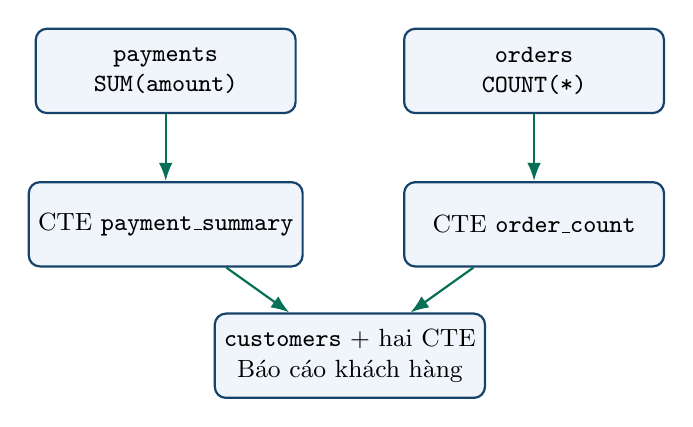
\begin{tikzpicture}[>=Latex,node distance=.7cm and 1.0cm,
 box/.style={draw=NEUBlue,thick,rounded corners,fill=NEUPale,minimum width=3.3cm,minimum height=1.07cm,align=center,font=\small}]
\node[box] (pay) {\texttt{payments}\\\texttt{SUM(amount)}};
\node[box,right=1.35cm of pay] (ords) {\texttt{orders}\\\texttt{COUNT(*)}};
\node[box,below=.85cm of pay] (paysum) {CTE \texttt{payment\_summary}};
\node[box,below=.85cm of ords] (ordcnt) {CTE \texttt{order\_count}};
\node[box,below=1.12cm of $(paysum)!0.5!(ordcnt)$] (final) {\texttt{customers} + hai CTE\\Báo cáo khách hàng};
\draw[->,thick,NEUGreen](pay)--(paysum);
\draw[->,thick,NEUGreen](ords)--(ordcnt);
\draw[->,thick,NEUGreen](paysum)--(final);
\draw[->,thick,NEUGreen](ordcnt)--(final);
\end{tikzpicture}
\end{center}
\end{frame}

\begin{frame}[fragile]{Hai CTE: khai báo và tính toán}
\small
\begin{lstlisting}[basicstyle=\ttfamily\scriptsize]
WITH
payment_summary AS (
    SELECT customerNumber,
           SUM(amount) AS totalPayment
    FROM payments GROUP BY customerNumber
),
order_count AS (
    SELECT customerNumber,
           COUNT(*) AS numberOfOrders
    FROM orders GROUP BY customerNumber
)
-- SELECT chinh nam o slide tiep theo
\end{lstlisting}
\vspace{.1em}
\begin{itemize}
\item Hai CTE đều có khóa \code{customerNumber}.
\item Không nối thẳng \code{payments} với \code{orders} để tránh nhân số bản ghi.
\end{itemize}
\end{frame}

\begin{frame}[fragile]{Hai CTE: truy vấn cuối}
\small
\begin{lstlisting}[basicstyle=\ttfamily\scriptsize]
-- Tiep sau phan WITH o slide truoc
SELECT c.customerNumber, c.customerName,
       ps.totalPayment, oc.numberOfOrders
FROM customers AS c
LEFT JOIN payment_summary AS ps
  ON c.customerNumber = ps.customerNumber
LEFT JOIN order_count AS oc
  ON c.customerNumber = oc.customerNumber;
\end{lstlisting}
\vspace{.1em}
\begin{itemize}
\item Đầu ra: mã khách, tên khách, tổng thanh toán, số đơn hàng.
\item \textbf{Đây là phần tiếp nối của cùng một câu lệnh WITH}; không chạy đoạn này riêng lẻ.
\item \code{LEFT JOIN}: giữ cả khách hàng chưa có đơn hoặc thanh toán.
\end{itemize}
\end{frame}

\begin{frame}[fragile]{Hai CTE xâu chuỗi: CTE 2 sử dụng CTE 1}
\small
\begin{lstlisting}[basicstyle=\ttfamily\scriptsize]
WITH order_totals AS (
  SELECT orderNumber,
         SUM(quantityOrdered*priceEach) AS total
  FROM orderdetails GROUP BY orderNumber
),
high_value AS (
  SELECT orderNumber, total
  FROM order_totals WHERE total > 50000
)
SELECT *
FROM high_value
ORDER BY total DESC;
\end{lstlisting}
\vspace{.1em}
\begin{itemize}
\item \code{order\_totals}: tính tổng của từng đơn.
\item \code{high\_value}: chọn đơn có tổng vượt ngưỡng.
\item Mô hình tách thành các bước có tên dễ đọc.
\end{itemize}
\end{frame}

\begin{frame}[fragile]{Thực hành 4: hai CTE tổng hợp}
\begin{block}{Yêu cầu}
Tạo \code{payment\_summary} và \code{order\_count}; nối với \code{customers} và hiển thị \code{customerName}, \code{totalPayment}, \code{numberOfOrders}.
\end{block}
\begin{alertblock}{Gợi ý làm bài}
\code{payment\_summary} từ \code{payments}; \code{order\_count} từ \code{orders}. Cả hai dùng \code{customerNumber}.
\end{alertblock}
\end{frame}

\section{CTE đệ quy: WITH RECURSIVE}

\begin{frame}[fragile]{Khi nào cần WITH RECURSIVE?}
\small
\begin{itemize}
\item Dữ liệu có cấu trúc nhiều cấp, chẳng hạn tổ chức nhân sự hoặc danh mục cha -- con.
\item Một hàng có thể tham chiếu hàng khác cùng bảng.
\item Không biết trước số cấp phải duyệt; cần tìm mức kế tiếp từ kết quả mức trước.
\item \code{WITH RECURSIVE} có thể mô tả quá trình mở rộng theo từng vòng.
\end{itemize}
\vspace{.3em}\begin{block}{Điểm cần nhớ}
Trong \code{classicmodels}: \code{employees.reportsTo} liên kết đến \code{employees.employeeNumber}.
\end{block}
\end{frame}

\begin{frame}[fragile]{Cấu trúc chuẩn của CTE đệ quy}
\small
\begin{lstlisting}[basicstyle=\ttfamily\scriptsize]
WITH RECURSIVE hierarchy AS (
    -- Anchor member: diem bat dau
    SELECT ...
    FROM source_table
    WHERE root_condition

    UNION ALL

    -- Recursive member: them cap ke tiep
    SELECT ...
    FROM source_table AS child
    JOIN hierarchy AS parent ON ...
)
SELECT * FROM hierarchy;
\end{lstlisting}
\vspace{.1em}
\begin{itemize}
\item \textbf{Anchor}: tạo tập kết quả ban đầu.
\item \textbf{Recursive member}: tham chiếu chính CTE và tạo dòng tiếp theo.
\item \code{UNION ALL}: kết hợp các dòng mới; cần điều kiện kết thúc hợp lý.
\end{itemize}
\end{frame}

\begin{frame}[fragile]{Cây quản lý minh họa}

\begin{center}
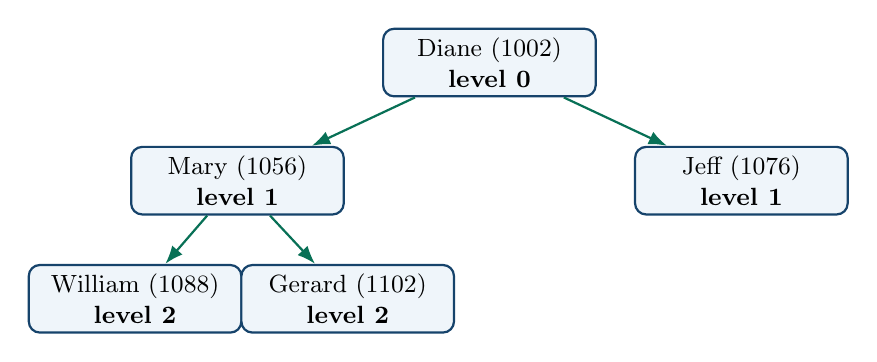
\begin{tikzpicture}[>=Latex, every node/.style={font=\small},
 emp/.style={draw=NEUBlue,thick,rounded corners,fill=NEUPale,minimum width=2.7cm,minimum height=.78cm,align=center}]
\node[emp] (ceo) at (6,3.6) {Diane (1002)\\\textbf{level 0}};
\node[emp] (a) at (2.8,2.1) {Mary (1056)\\\textbf{level 1}};
\node[emp] (bb) at (9.2,2.1) {Jeff (1076)\\\textbf{level 1}};
\node[emp] (c) at (1.5,.6) {William (1088)\\\textbf{level 2}};
\node[emp] (d) at (4.2,.6) {Gerard (1102)\\\textbf{level 2}};
\draw[->,thick,NEUGreen](ceo)--(a);
\draw[->,thick,NEUGreen](ceo)--(bb);
\draw[->,thick,NEUGreen](a)--(c);
\draw[->,thick,NEUGreen](a)--(d);
\end{tikzpicture}
\end{center}
\small\textbf{Lưu ý:} tên và mã nhân viên trong hình là ví dụ minh họa cho cấu trúc \code{reportsTo}; thứ tự các cấp được tính từ gốc.
\end{frame}

\begin{frame}[fragile]{employees: dữ liệu minh họa}
\small
\begin{center}
\begin{tabular}{l l l}
\toprule
employeeNumber & firstName & reportsTo \\
\midrule
1002 & Diane & \code{NULL} \\
1056 & Mary & 1002 \\
1076 & Jeff & 1002 \\
1088 & William & 1056 \\
1102 & Gerard & 1056 \\
\bottomrule
\end{tabular}
\end{center}
\vspace{.25em}
\small Bản ghi gốc thỏa \code{reportsTo IS NULL}. Một nhân viên ở cấp $k+1$ có \code{reportsTo} bằng \code{employeeNumber} của nhân viên ở cấp $k$.
\end{frame}

\begin{frame}[fragile]{CTE đệ quy: phần anchor}
\small
\begin{lstlisting}[basicstyle=\ttfamily\scriptsize]
WITH RECURSIVE employee_hierarchy AS (
  SELECT employeeNumber, firstName,
         lastName, reportsTo, jobTitle,
         0 AS level
  FROM employees
  WHERE reportsTo IS NULL

  UNION ALL
  -- Recursive member o slide tiep theo
)
SELECT * FROM employee_hierarchy;
\end{lstlisting}
\vspace{.1em}
\begin{itemize}
\item \code{reportsTo IS NULL}: xác định nhân viên gốc.
\item \code{0 AS level}: cấp gốc.
\item Đoạn code này là \textbf{minh họa cấu trúc chưa hoàn chỉnh}; xem tiếp phần đệ quy.
\end{itemize}
\end{frame}

\begin{frame}[fragile]{CTE đệ quy: phần recursive member}
\small
\begin{lstlisting}[basicstyle=\ttfamily\scriptsize]
-- Recursive member ben trong CTE
SELECT e.employeeNumber, e.firstName,
       e.lastName, e.reportsTo, e.jobTitle,
       eh.level + 1 AS level
FROM employees AS e
JOIN employee_hierarchy AS eh
  ON e.reportsTo = eh.employeeNumber
\end{lstlisting}
\vspace{.1em}
\begin{itemize}
\item Nhân viên \code{e} là \textbf{con} của nhân viên đã có trong \code{eh}.
\item \code{eh.level + 1}: cấp mới = cấp của quản lý + 1.
\item Mỗi vế của \code{UNION ALL} phải có cùng số cột và kiểu tương thích.
\end{itemize}
\end{frame}

\begin{frame}[fragile]{Truy vấn hoàn chỉnh: cây quản lý}
\small
\begin{lstlisting}[basicstyle=\ttfamily\scriptsize]
WITH RECURSIVE h AS (
  SELECT employeeNumber, firstName, lastName,
         reportsTo, 0 AS level
  FROM employees WHERE reportsTo IS NULL
  UNION ALL
  SELECT e.employeeNumber, e.firstName,
         e.lastName, e.reportsTo, h.level+1
  FROM employees AS e
  JOIN h ON e.reportsTo=h.employeeNumber
)
SELECT employeeNumber, firstName,
       lastName, level FROM h
ORDER BY level, employeeNumber;
\end{lstlisting}
\vspace{.1em}
\begin{itemize}
\item Đầu ra có \code{employeeNumber}, \code{firstName}, \code{lastName}, \code{level}.
\item \code{ORDER BY level, employeeNumber} sắp xếp kết quả sau khi tạo phân cấp.
\end{itemize}
\end{frame}

\begin{frame}[fragile]{CTE đệ quy chạy theo các vòng như thế nào?}

\small
\begin{tabularx}{\linewidth}{>{\bfseries}l X X}
\toprule
Vòng & Thành viên vừa tìm được & Giải thích\\\midrule
$0$ & \texttt{Diane / 1002 / level 0} & Anchor: \texttt{reportsTo IS NULL}.\\
$1$ & \texttt{Mary, Jeff / level 1} & Các nhân viên có \texttt{reportsTo=1002}.\\
$2$ & \texttt{William, Gerard / level 2} & Tìm nhân viên báo cáo cho người ở vòng 1.\\
$3$ & Không thêm dòng mới & Kết thúc, nếu không còn cấp dưới.\\
\bottomrule
\end{tabularx}
\vspace{.4cm}
\begin{block}{Diễn giải logic}
Ở mỗi bước, thành viên đệ quy thêm các nhân viên thuộc cấp kế tiếp, đến khi không còn bản ghi mới được sinh ra.
\end{block}
\end{frame}

\begin{frame}[fragile]{Lọc theo level sau CTE}
\small
\begin{lstlisting}[basicstyle=\ttfamily\scriptsize]
WITH RECURSIVE h AS (
  SELECT employeeNumber, reportsTo,
         0 AS level
  FROM employees WHERE reportsTo IS NULL
  UNION ALL
  SELECT e.employeeNumber, e.reportsTo,
         h.level + 1
  FROM employees e
  JOIN h ON e.reportsTo=h.employeeNumber
)
SELECT employeeNumber, reportsTo, level
FROM h WHERE level >= 2;
\end{lstlisting}
\vspace{.1em}
\begin{itemize}
\item Điều kiện ở ngoài \code{WHERE level >= 2} chỉ ẩn các cấp 0--1 khỏi kết quả cuối.
\item Nó không thay anchor hay điều kiện duyệt phân cấp.
\end{itemize}
\end{frame}

\begin{frame}[fragile]{Giới hạn độ sâu để tăng an toàn}
\small
\begin{lstlisting}[basicstyle=\ttfamily\scriptsize]
WITH RECURSIVE h AS (
  SELECT employeeNumber, reportsTo,
         0 AS level
  FROM employees WHERE reportsTo IS NULL
  UNION ALL
  SELECT e.employeeNumber, e.reportsTo,
         h.level+1
  FROM employees e JOIN h
    ON e.reportsTo=h.employeeNumber
  WHERE h.level < 5
)
SELECT * FROM h;
\end{lstlisting}
\vspace{.1em}
\begin{itemize}
\item Đặt điều kiện \code{h.level < 5} ngay trong \textbf{recursive member}.
\item Bảo đảm không duyệt sâu hơn \code{level 5} (nếu gốc là cấp 0).
\item Không thay thế nhu cầu kiểm tra chu trình trong dữ liệu.
\end{itemize}
\end{frame}

\begin{frame}[fragile]{Điều gì làm CTE đệ quy dừng lại?}
\small
\begin{itemize}
\item Thành viên đệ quy không tạo thêm dòng nào \textbf{hoặc} giới hạn đệ quy được áp dụng.
\item Nối sai có thể sinh lặp vô hạn / bùng nổ số dòng.
\item Dữ liệu có chu trình cần cơ chế phát hiện các node đã đi qua nếu muốn xử lý tổng quát.
\item MySQL có biến \code{cte\_max\_recursion\_depth} giới hạn số mức lặp mặc định (thường là 1000).
\end{itemize}
\vspace{.3em}\begin{block}{Điểm cần nhớ}
Đối với cây nhân sự hợp lệ có một gốc, quan hệ \code{reportsTo} phải tránh chu trình và thường nên có khóa ngoại tự tham chiếu.
\end{block}
\end{frame}

\begin{frame}[fragile]{Thực hành 5: truy vấn phân cấp}
\begin{block}{Yêu cầu}
Viết CTE đệ quy trả về \code{employeeNumber}, \code{firstName}, \code{lastName}, \code{jobTitle}, \code{level} cho cây \code{employees}.
\end{block}
\begin{alertblock}{Gợi ý làm bài}
Anchor: \code{reportsTo IS NULL}; recursive JOIN: \code{e.reportsTo = h.employeeNumber}; cấp tăng thêm 1.
\end{alertblock}
\end{frame}

\section{So sánh và các lỗi thường gặp}

\begin{frame}[fragile]{So sánh các hình thức CTE}
\small
\begin{center}
\begin{tabular}{l l p{3.4cm}}
\toprule
Hình thức & Khai báo & Mục đích \\
\midrule
CTE thường & \code{WITH name AS (...)} & Kết quả trung gian \\
Nhiều CTE & \code{WITH a AS (...), b AS (...)} & Chia nhiều bước \\
CTE đệ quy & \code{WITH RECURSIVE name AS (...)} & Cấu trúc phân cấp \\
\bottomrule
\end{tabular}
\end{center}
\vspace{.25em}
\small Có thể kết hợp với \code{WHERE}, \code{JOIN}, \code{GROUP BY}, \code{ORDER BY} và \code{LIMIT}.
\end{frame}

\begin{frame}[fragile]{Lỗi 1: thiếu dấu phẩy giữa hai CTE}
\small
\begin{lstlisting}[basicstyle=\ttfamily\scriptsize]
-- SAI: thieu dau phay giua a va b
WITH a AS (SELECT * FROM orders)
b AS (SELECT * FROM customers)
SELECT * FROM a;

-- DUNG: co dau phay
WITH a AS (SELECT * FROM orders),
     b AS (SELECT * FROM customers)
SELECT * FROM a;
\end{lstlisting}
\vspace{.1em}
\begin{itemize}
\item Trong một \code{WITH} có nhiều CTE, ngăn cách bằng \textbf{dấu phẩy}.
\item Mỗi CTE có một tên và một định nghĩa trong dấu ngoặc tròn.
\end{itemize}
\end{frame}

\begin{frame}[fragile]{Lỗi 2: quên câu truy vấn chính}
\small
\begin{lstlisting}[basicstyle=\ttfamily\scriptsize]
-- SAI: WITH khong the ket thuc mot minh
WITH usa_customers AS (
  SELECT * FROM customers
  WHERE country='USA'
);

-- DUNG: them truy van su dung CTE
WITH usa_customers AS (
  SELECT * FROM customers
  WHERE country='USA'
)
SELECT * FROM usa_customers;
\end{lstlisting}
\vspace{.1em}
\begin{itemize}
\item \code{WITH} không phải lệnh tạo bảng riêng lẻ.
\item CTE phải được theo sau bởi một câu lệnh hợp lệ sử dụng nó.
\end{itemize}
\end{frame}

\begin{frame}[fragile]{Lỗi 3: tên CTE trùng tên bảng}
\small
\begin{lstlisting}[basicstyle=\ttfamily\scriptsize]
-- Kho doc va co the gay nham lan
WITH customers AS (
  SELECT * FROM customers
  WHERE country='USA'
)
SELECT * FROM customers;

-- Nen dat ten mo ta nghiep vu
WITH usa_customers AS (
  SELECT * FROM customers
  WHERE country='USA'
)
SELECT * FROM usa_customers;
\end{lstlisting}
\vspace{.1em}
\begin{itemize}
\item Dùng tên riêng mô tả chức năng CTE.
\item Tránh đụng tên bảng gốc hoặc tên CTE đã tồn tại trong cùng phạm vi.
\end{itemize}
\end{frame}

\begin{frame}[fragile]{Lỗi 4: điều kiện JOIN sai trong CTE đệ quy}
\small
\begin{lstlisting}[basicstyle=\ttfamily\scriptsize]
-- DUNG: child.reportsTo = parent.employeeNumber
JOIN employee_hierarchy AS parent
  ON e.reportsTo = parent.employeeNumber

-- SAI trong bai toan nay:
JOIN employee_hierarchy AS parent
  ON e.employeeNumber = parent.employeeNumber
\end{lstlisting}
\vspace{.1em}
\begin{itemize}
\item Nếu tự nối theo \code{employeeNumber} ở cả hai phía, truy vấn không đi sang con.
\item Điều kiện đúng phải liên kết \code{reportsTo} của nhân viên với mã người quản lý.
\end{itemize}
\end{frame}

\begin{frame}[fragile]{Lỗi 5: UNION ALL vs UNION}
\small
\begin{lstlisting}[basicstyle=\ttfamily\scriptsize]
WITH RECURSIVE h AS (
  SELECT employeeNumber, reportsTo,
         0 AS level
  FROM employees WHERE reportsTo IS NULL
  UNION ALL
  SELECT e.employeeNumber, e.reportsTo,
         h.level+1
  FROM employees e
  JOIN h ON e.reportsTo=h.employeeNumber
)
SELECT * FROM h;
\end{lstlisting}
\vspace{.1em}
\begin{itemize}
\item \code{UNION ALL} giữ các dòng sinh ra; thường phù hợp với cây đơn giản.
\item \code{UNION} loại dòng trùng, nhưng không bảo đảm loại được chu trình nếu \code{level} liên tục tăng.
\item Không tự động coi \code{UNION} là cơ chế chống vòng lặp an toàn.
\end{itemize}
\end{frame}

\begin{frame}[fragile]{Các lưu ý về hiệu năng}
\small
\begin{itemize}
\item CTE ưu tiên khả năng diễn đạt; không mặc định giúp tăng hiệu năng.
\item Lọc các cột/dòng cần thiết và đặt chỉ mục trên khóa JOIN được sử dụng nhiều.
\item \code{EXPLAIN} để quan sát kế hoạch thực thi thay vì suy đoán.
\item Với truy vấn phân cấp lớn: giới hạn độ sâu, kiểm tra chu trình, và tránh mở rộng không cần thiết.
\end{itemize}
\vspace{.3em}\begin{block}{Điểm cần nhớ}
Ở MySQL, việc optimizer gộp hay materialize CTE tùy trường hợp và phiên bản; không nên khẳng định CTE luôn là bảng tạm vật lý.
\end{block}
\end{frame}

\section{Tổng kết và tự luyện}

\begin{frame}[fragile]{Tự luyện A: tổng thanh toán}
\begin{block}{Yêu cầu}
Dùng CTE đếm số khoản thanh toán và tính tổng tiền theo \code{customerNumber}; chỉ trả các khách có tổng tiền trên 50000.
\end{block}
\begin{alertblock}{Gợi ý làm bài}
Bảng nguồn \code{payments}; cột sử dụng \code{customerNumber}, \code{amount}; đặt bí danh cho \code{COUNT(*)} và \code{SUM(amount)}.
\end{alertblock}
\end{frame}

\begin{frame}[fragile]{Tự luyện B: top doanh thu sản phẩm}
\begin{block}{Yêu cầu}
Từ \code{orderdetails}, tạo CTE tính doanh thu theo \code{productCode}; nối với \code{products} để lấy \code{productName}.
\end{block}
\begin{alertblock}{Gợi ý làm bài}
Doanh thu từng dòng = \code{quantityOrdered * priceEach}. Gom theo \code{productCode}, sau đó JOIN theo \code{productCode}.
\end{alertblock}
\end{frame}

\begin{frame}[fragile]{Tự luyện C: nhiều CTE}
\begin{block}{Yêu cầu}
Hiển thị \code{customerName}, \code{numberOfOrders}, \code{totalPayment}; giữ cả khách hàng chưa từng thanh toán.
\end{block}
\begin{alertblock}{Gợi ý làm bài}
Tạo 2 CTE riêng từ \code{orders} và \code{payments}; dùng \code{customers LEFT JOIN ...}.
\end{alertblock}
\end{frame}

\begin{frame}[fragile]{Tự luyện D: quản lý nhân viên}
\begin{block}{Yêu cầu}
Viết CTE đệ quy cho cấp quản lý và chỉ hiển thị nhân viên ở cấp ít nhất 2.
\end{block}
\begin{alertblock}{Gợi ý làm bài}
Giữ phần anchor và recursive member đầy đủ; đặt \code{WHERE level >= 2} ở truy vấn chính.
\end{alertblock}
\end{frame}

\begin{frame}[fragile]{Tổng kết: 6 ý chính}

\begin{enumerate}
\item CTE là \textbf{kết quả trung gian có tên} trong phạm vi câu lệnh.
\item Cú pháp cơ bản: \code{WITH name AS (SELECT ...)}.
\item CTE kết hợp tự nhiên với \code{WHERE}, \code{ORDER BY}, \code{LIMIT}.
\item Tổng hợp \code{GROUP BY} trong CTE rồi \code{JOIN} với bảng mô tả.
\item Nhiều CTE giúp chia báo cáo thành các bước rõ ràng.
\item \code{WITH RECURSIVE} gồm \textbf{anchor + recursive member}; dùng duyệt phân cấp.
\end{enumerate}
\vspace{.3em}
\begin{block}{Tự học}
Lab tương tác SELECT 6: làm đủ 45 bài, xem schema và thử \code{Run / Check} cho các truy vấn.
\end{block}
\end{frame}

\begin{frame}[fragile]{Tài liệu và bài tập}

\small
\textbf{Nguồn bài giảng:}
\begin{itemize}
\item \url{https://vudmvn.github.io/dbms-course/lectures/MySQL/querying-data/select/select-statement-6/}
\end{itemize}
\vspace{.4cm}
\textbf{Các kỹ năng nên đạt:}
\begin{enumerate}
\item Xác định cột nguồn trước khi viết \texttt{SELECT}.
\item Xác định khóa nhóm hoặc khóa nối trước khi viết CTE.
\item Phân biệt câu lệnh cuối với các định nghĩa CTE.
\item Duyệt đúng cây quản lý, nhận diện anchor/recursive member.
\end{enumerate}
\end{frame}

\end{document}
